\documentclass[spanish]{article}
\usepackage[spanish]{babel}
\usepackage{amsmath}
\usepackage{amssymb}
\usepackage[utf8]{inputenc}
\usepackage{vmargin}
\usepackage{graphicx}


\begin{document}
	\setpapersize{USletter}
	\setmarginsrb{30mm}{30mm}{30mm}{30mm}{0pt}{0mm}{0pt}{0mm}
	
	\begin{center}
	{\Large Análisis de Algoritmos, Sem: 2018-1, 3CV2 Práctica 1, 24-Agosto-2017}\\
{\huge {\bf Práctica 1: Determinación experimental de
la complejidad de un algoritmo}} \\
{\large {\bf Martínez Berumen Luis Daniel}\\
Escuela Superior de Cómputo \\
Instituto Politécnico Nacional}\\
dany.berumen@gmail.com\\	
	\end{center}
	\bigskip
	
	\bigskip
	
	\bigskip
En el presente trabajose analizará, por medio de  la
 experimentación, la complejidad de un  algoritmo dado,  proponiendo  una 
función g(n) tal que S $\in$ O(g(n)) y g(n) sea mínima, en el sentido 
de que si S $\in$ O(h(n)), entonces g(n) $\in$ O(h(n)). 
A través de la observación se compará el  comportamiento entre 
el tiempo de ejecución y un número de veces que se ejecuta una función.
\bigskip


	{\Large {\bf Palabras Clave}}\\
	\begin{itemize}
		\item Algoritmo
		\item Complejidad
		\item Experimentacion
		\item Eficiencia
	\end{itemize}
	\bigskip
	
	\section{Introducci\'on}
	En los tiempos actuales es importante la manera en la que resolvemos los trabajos diariamente, por medio de diferentes acciones que pueden llegar a ser repetitivas se logran resolver la mayoria de los problemas que enfrentamos diariamente.
	Es por eso que es importante el estudio de los algoritmos empleados día con día para así determinar los que nos permitan resolver nuestro trabajo de la manera más optima posible.
	Al igual que nuestro trabajo, los algoritmos que usamos pueden ser empleados para automatizar diferentes aspectos de nuestras actividades cotidianas, o hasta trabajos de grandes industrias. 
	Empleando el algoritmo que mejor se adecue al trabajo a realizar, se lograra tener tiempos menores, lo que se podria traducir en ahorros en produccion y aumento en la eficiencia.
	\bigskip
\newpage
	\section{Conceptos B\'asicos}
	Es necesario definir algunos terminos para la comprension de el analicis efectuado a continuacion, tales como $\theta$, O y $\Omega$.\\
	 	$\theta$(n):\\
		Sea g(n) una función. Se define  $\theta$ (g(n)) como:\\
		
		 	$\theta$(g(n)) = $\{ f(n) \quad | \quad \exists c1,c2>0 \quad \& \quad n_{0}>0 \quad \mid \quad \forall n>=n_{0} \quad 0<= c1g(n) <= f(n) <= c2g(n) \}$
	\bigskip		 	
		 	
	O(n):\\
		Sea  g(n)  una función, O(n) se define como:\\
		
			\hspace{1cm}O(n)=$\{f(n) \quad | \quad \exists c >0 \quad \& \quad n_{0}>0 \quad | \quad f(n) <= Cg(n) \quad \forall  n>= n_{0} \}$
	\bigskip
	
	$\Omega$(n):\\
	Sea  g(n)  una función. Se define $\Omega$ (g(n)) como:\\

		\hspace{1cm}$\Omega$(g(n)) =$\{f(n) \quad | \quad \exists c >0 \quad \& \quad n_{0}>0 \quad \mid \quad  0<= cg(n)<= f(n) \quad \forall n>= n_{0} \}$
	\bigskip

	Se muestra experimentalmente el tiempo computacional de dos algoritmos y un tercero de manera teórica, 
	el primer algoritmo de desarrollo experimental consiste en sumar dos números enteros en notación binariaconsiderando que: 
	Dos arreglos unidimensionales A de tamaño n y B de tamaño m con k = $\log_{2}(n)$ y t = $\log{2}(m)$ almacenarán los números a sumar. 
	La suma se almacenará en un arreglo C. El propósito es obtener el tiempo que se tarda en realizar dicha operación con un tamaño r que se le asigna al arreglo.
	



\begin{itemize}
	\item 0+0=0
	\item 0+1=1
	\item 1+0=1
	\item 1+1=0 y se acarrea un 1 que se sumara a la siguiente posicion
	\item Con esto podemos aclarar 4 casos:
	\item cuando la suma da 0: se agrega un 0 al arreglo C
	\item cuando la suma da 1: se agrega un 1 al arreglo C
	\item cuando la suma da 2: se agrega un 0  al arreglo C y el acarreo se hace 1
	\item cuando la suma da 3: se agrega un 1 al arreglo C y el acarreo se hace 1
\end{itemize}

El segundo ejercicio trata de la implementacion del algoritmo de Euclides para encontrar el maximo comun divisor de dos números enteros positivos m y n. 
Con el finn deobtener el tiempo de ejecución cuando se mande a llamar la función de Euclides, 
pero con la condición que los números a los cueles se obtendrá el m.c.d 
\\\\
Para el algoritmo teórico se encontrará la complejidad de un programa de ordenamiento.
	
	\newpage
\section{Experimentaci\'on y Resultados}
	\subsection{Suma Binaria}
	Suma (A,B,n[1,...,17],c)\\
Entrada: i[1,..., 17]\\
Salida: Tiempo computacional de n[1,...,17]\\
1. for i $\leftarrow$ 1 to i $\leftarrow$ 17 do\\
2.		\hspace{0.7cm}n $\leftarrow$ potencia(2,i)\\
3.      \hspace{0.7cm}suma(A,B,n,c)\\
4. 		\hspace{0.7cm}print(c)
\bigskip

	{\large{\bf-Mostrar la grafica para la función S que muestre tiempo vs r con r = m = n (considere diversos valores de r).}}\\
	\begin{center}
		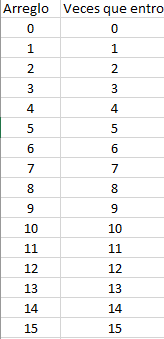
\includegraphics{tabla1}
		\\Figura 1\\
	\end{center}
	\newpage
	Cuya grafica es es:\\
	\begin{center}
		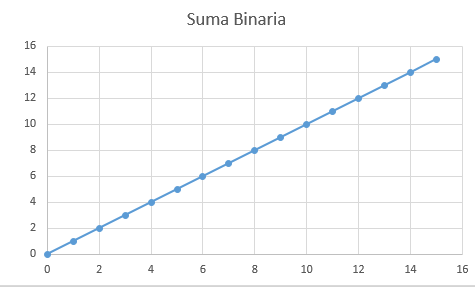
\includegraphics{sumaBinaria}\\
		Figura 2\\
	\end{center}
	{\large{\bf -Proponer una función g(n) tal que S $\in$ O(g(n)) y g(n) sea mínima, en el sentido de que si S $\in$  O(h(n)), entonces g(n) $\in$  O(h(n)).}}\\
	Por los resultados obtenidos en la última gráfica proponemos que la complejidad del algoritmo S es de tipo lineal, y se propone la función O(n).
	\bigskip
	
	{\large {\bf -Conclusiones}}\\
	{\bf En este experimento se pudo comprobar el como se efectua una suma binaria, aunque en cuestiones de tiempo, no marco diferencia al meter grandes arreglos, supongo que el algoritmo empleado fue una buena solucion, veo que los tamaños no importan mucho en este problema o no con la computadora donde fueron programados. \\

	\newpage
	\subsection{Euclides}
	{\large{\bf1.- Pseudoc\'odigo Algoritmo de Euclides}}\\
	Euclides (A,B,c]\\
Entrada: fibonacci(n),fibonacci(n-1) con $1<=n<50$\\
Salida: Tiempo computacional de $1<=n<50$\\
1.  for i $\leftarrow$ 1 to i $\leftarrow$ 79 do\\
2.      \hspace{0.7cm}a $\leftarrow$ fibonacci(i)\\
3.      \hspace{0.7cm}b $\leftarrow$ fibonacci(i+1)\\
4.      \hspace{0.7cm}e $\leftarrow$ euclides(b,a,c)\\
5.	   \hspace{0.7cm}print(c)\\

\bigskip

	{\large{\bf -Mostrar diversas gráficas para la función Euclides que muestre tiempo vs diferentes valores de m y n.}}\\
	Para para los primeros 79 valores de Fibonacci:
	\begin{center}
		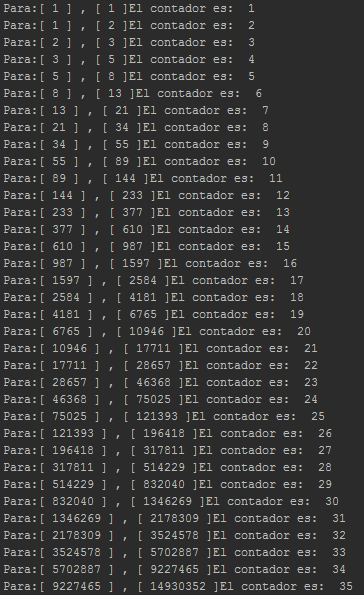
\includegraphics{fibo1}\\
		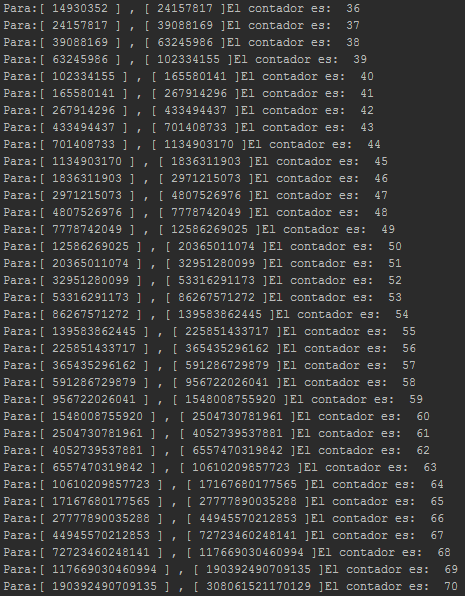
\includegraphics{fibo2}\\
		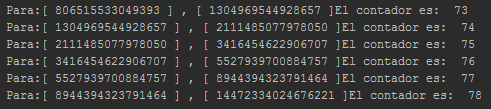
\includegraphics{fibo3}\\
		Figura 3\\
	\end{center}

	La gráfica es:\\
	\begin{center}
		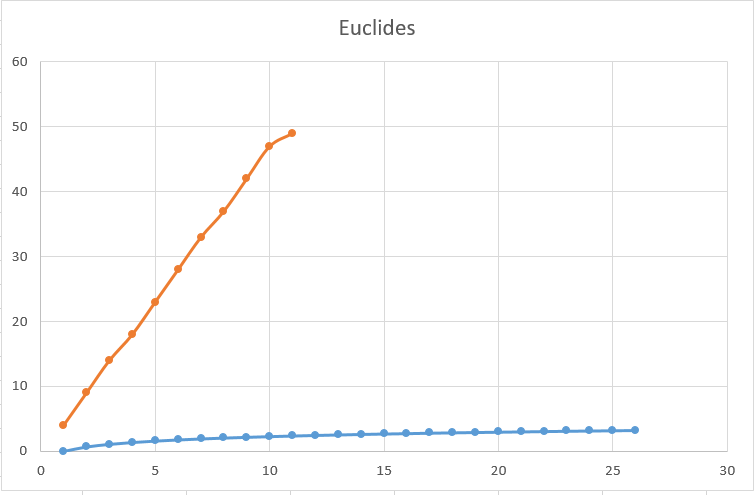
\includegraphics{euclides}\\
		Figura 4\\
	\end{center}

	{\large{\bf -Proponer una función g(n) tal que Euclides $\in$ O(g(n)) y g(n) sea mínima, en el sentido de que si Euclides $\in$  O(h(n)), entonces g(n) $\in$  O(h(n)).}}\\
	Por los resultados obtenidos en la última gráfica proponemos que la complejidad del algoritmo Euclides es de tipo logarítmica y propones la función O($\log_{2}(n)$) ya que O($\log_{2}(n)$) pasa ser cota superior cumpliendo así la definición de O($\log_{2}(n)$).
	\bigskip

	{\large {\bf -Conclusiones}}\\
	No creia que el algoritmo de Euclides fuera de tipo logaritmico, la cuestion de los tiempos es algo comnplicado de medir, al menos para mi nivel de programacion actual, para solucuionar esto, implemente un contador en las veces que entraba a la funcion, siendo esta la mejor forma para lograr contabilizar el tiempo computable.
	\newpage
	\section{Conclusi\'on General}
	Como lo mencione al principio del trabajo, los algoritmos son uina herramienta que ocupamos todos en nuestro dia a dia, por eso es importante encontrar la manera de analizar estos algoritmos y determinar si son la mejor solucion a nuestras necesidades, con este comienzo vemos que el analisis de algoritmos no es cosa de gracia, es un tema bastante complejo que requiere de mucha atencion.
	\newpage
	\section{Anexos}
	
	{\Large{\bf Select-Sort}}\\
	Select-Sort(A[0...n-1]) \hspace{2.9cm}Costo \hspace{1.7cm} \#Pasos \\
	1.-	\hspace{0.7cm}for j $\leftarrow$ 0 to n-2 do \hspace{2.3cm} C1 \hspace{2.0cm} n\\
	2.-		\hspace{1.4cm}k $\leftarrow$ j\hspace{4.1cm}   C2 \hspace{2.0cm} n-1\\
	3.-		\hspace{1.4cm}for i $\leftarrow$ j+1 to n-1 do \hspace{1.1cm} C3 \hspace{2.0cm}$\sum_{i=0}^{n-1}t_{i}$\\
	4.-			\hspace{2.1cm}if A[i] $<$ A[k] then \hspace{1cm} C4 \hspace{2.0cm}$\sum_{i=0}^{n-1}(t_{i}-1)$\\
	5.-				\hspace{2.8cm}k $\leftarrow$ i \hspace{2.5cm} C5 \hspace{2.0cm}$\sum_{i=0}^{n-1}R_{i}$\\
	6.-	\hspace{1.4cm} intercambia(A[j],A[k]) \hspace{1.2cm} C6 \hspace{2.0cm}n-1\\
	\bigskip
	
	\bigskip
	
	El peor de los casos se presenta cuando el arreglo esta ordenado en forma decreciente por lo  que:\\ 
	$t_{i} = n-i$ y\\
	$R_{i} = n-i-1 = t_{i}-1$\\
	\bigskip
	
	Por lo tanto tenemos que:\\
	T(n) = C1n + C2(n-1) + C3($\sum_{i=0}^{n-1}(n-i)$) + C4($\sum_{i=0}^{n-1}(n-i-1)$) + C5($\sum_{i=0}^{n-1}(n-i-1)$) + C6(n-1)
	\bigskip
	
	T(n) = C1n + C2n -C2 + C3($\sum_{i=0}^{n-1}n$) - C3($\sum_{i=0}^{n-1}i$) + C4($\sum_{i=0}^{n-1}n$) - C4($\sum_{i=0}^{n-1}i$) - C4($\sum_{i=0}^{n-1}1$) + C5($\sum_{i=0}^{n-1}n$) -C5 ($\sum_{i=0}^{n-1}i$) - C5($\sum_{i=0}^{n-1}1$) + C6n -C6
	\bigskip
	
	T(n) = (C1+C2+C6)n + (C3+C4+C5)($n^{2}$) - (C3+C4+C5)($\sum_{i=1}^{n}(i-1)$) - (C4+C5)n -(C2+C6)
	\bigskip
	
	T(n) = (C3+C4+C5)$n^{2}$ -(C3+C4+C5)($\dfrac{n(n+1)}{2}$ - n) +(C1+C2-C4-C5+C6)n - (C2+C6)
	\bigskip
	
	T(n) = ($\dfrac{C3+C4+C5}{2}$)$n^{2}$	+ (C1+C2+C3+C6)n - (C2+C6)
	\bigskip
	
	$\therefore$
	$ T(n) \quad \in \quad O(n^{2})$
	\bigskip	
	
	\section{Bibliografía}
	\begin{itemize}
		\item Brassard, G. (1997). Fundamentos de Algoritmia. España: Ed. Prentice Hall. ISBN 
	\end{itemize}
	
\end{document}